\chapter{Handling Cache Interference in Safety-Critical Systems}
\label{cha:handling_it}
This chapter explores existing solutions to the issue of the interference
generated by cache coherence in safety-critical systems. Three approaches are
considered: Limiting either the capabilities of either the architecture or the
software running on it in order to limit the generation of these interference
(Section~\ref{sec:rel_work:handling_it:through_restrictions}); Modifying the
architecture's hardware or adding new hardware components in order to lessen
the unpredictability (Section~\ref{sec:rel_work:handling_it:through_hardware});
and lastly, solutions that involve running software in safety-critical systems
by showing that the effects of the interference remain acceptable.

\section{Through Restrictions}
\label{sec:rel_work:handling_it:through_restrictions}
The crudest approach to the handling of interference generated by cache
coherence is to not have any because all caches are disabled. While this
solution tremendously improves the predictability of the system, it also
tremendously decreases its execution speed, to the point where it may be
preferable to use a single-core architecture with caches instead.

One step above is a solution in which the caches are enabled, but their content
is locked, making their usefulness severely limited but without compromising the
system's predictability.

In this section are presented strategies that allow the use of caches in a
limited manner in order to achieve reasonable execution speed while keeping the
system as predictable as possible.

\subsection{Shared Cache Partitioning}
\cite{10.1145/1629335.1629369} presents two algorithms for a condition
sufficient to prove schedulability, it is meant for tasks with time and cache
space constraints in the context of a shared L2 cache in which space is
partitioned in order to avoid contentions.  Thus, this work is more about
proving that the measures taken in order to address interference are sufficient
rather than a strategy to control the interference itself. For these
schedulability tests, the tasks are assumed to be non-preemptive and to have a
fixed priority.

The paper's first algorithm is based on constraint programming. It basically
considers that there is a task missing its deadline, which implies that either
all cores are being used, or that too little cache space is available.
Intervals at which either of these conditions is true are searched for in order
to find their maximal impact of the hypothetical task that missed its deadline.
If this maximum impact is lower than the slack (longest affordable delay) of
this hypothetical task, then the tasks are schedulable. The second algorithm is
very similar, but simplifies the constraints by simply assuming the worst
possible interference from the other tasks in all criteria with much less
regard for whether the configuration leading to this interference is actually
possible. This effectively creates a more scalable schedulability test, at the
cost of being much more pessimistic.

\stopallthesefloats
\subsection{Cache Coloring to Curtain Interference}
\begin{figure}[hbt]
\begin{center}
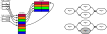
\includegraphics[width=\textwidth]{\chapterdirectory/figure/handling_it/cache_coloring_wcet.pdf}
\end{center}
\caption{Cache coloring aware scheduling, from \cite{DBLP:journals/corr/abs-1903-09310}}%
\label{fig:handling_it:cache_coloring}
\end{figure}
When using a set-associative cache, the cache is divided in equal sets of cache
lines. The memory element's physical address determines which of these sets of
cache lines it will go to. The cache eviction policy then applies solely inside
that set. The idea behind cache coloring is to exploit this, by determining
which memory element will find itself in which set of lines, and assigning
virtual addresses to physical addresses in a manner that will ensure a maximum
of virtual addresses will find themselves in the cache.

\cite{DBLP:journals/corr/abs-1903-09310} uses cache coloring in the opposite
manner. It instead assigns a single color (thus, set of cache lines) per
program. While this is not an efficient use of the cache for any one program,
it means that each program is effectively curtained into the set of caches of
its color. Using careful scheduling, the number of programs running in parallel
that share the same colors can be reduced (see
Figure~\ref{fig:handling_it:cache_coloring}), thus removing the interference
they can inflict on one another.
\stopallthesefloats

\subsection{Limited Shared Resources}
\begin{figure}
\centering
\includegraphics[width=0.6\columnwidth]{\chapterdirectory/figure/handling_it/marthy.png}
\caption{%
System running Marthy (Control Software in the figure), a figure extracted from
\cite{7311481}.
}
\label{fig:handling_it:marthy}
\end{figure}

One approach to dealing with cache coherence in multi-core processors for
environments requiring certification is to simply use the caches in a manner
that cancels the need for such a feature. Indeed, since the applications for
single core are already available, it stands to reason plenty of them could run
on multi-core processors without the need for shared memory elements. For
example, \cite{jean:tel-01341758} presents \textit{Marthy} (see
Figure~\ref{fig:handling_it:marthy}), a hypervisor aiming to enforce robust
partitioning between applications running on a COTS multi-core processor. This
hypervisor permanently lives in the cache of each core, using cache locking
mechanisms to avoid being inadvertently removed, and makes use of the MMU to
take over whenever an instruction triggers a cache miss, stalling that
instruction until access to the system's shared resources (i.e.~any shared
component, not just memory) is exclusively granted to the core by a TDMA. All
shared memory elements must be read-only, which does indeed remove the need for
cache coherence mechanisms.

\stopallthesefloats

\subsection{Isolated Communications Through Scheduling}
\begin{figure}
\centering
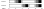
\includegraphics[width=0.5\columnwidth]{\chapterdirectory/figure/handling_it/deterministic_execution_model.pdf}
\caption{%
Overview of the strategy presented in \cite{10.1007/978-3-642-28293-5_9} (taken
from the paper)
}
\label{fig:handling_it:deterministic_execution_model}
\end{figure}

In \cite{10.1007/978-3-642-28293-5_9}, careful scheduling is used to make
calculating the worst-case execution time easier. This scheduling requires
programs running on each cores to have been sliced into computation blocks and
communication ones. Computation blocks are built so that while a core is in
one, the other cores cannot access the same data (or only as a read-only copy
if all tasks are only reading this data). Communications nodes indicate
fetching and writing periods (no computation), which are similarly limited by
any task currently performing a computation block. The paper provides a
strategy to automatically slice the programs intended for a core into a
scheduling of these types of blocks.
Figure~\ref{fig:handling_it:deterministic_execution_model} shows an example of
two cores having their tasks scheduled in this manner. White blocks indicate
time reserved for computation; grey blocks are for flushes; and black blocks
are for fetches.

Because they do not access any shared resource, calculating the worst-case
execution time of the computation blocks is equivalent to doing so on a single
core processor. \cite{10.1007/978-3-642-28293-5_9} proposes a solution for the
calculation of the worst-case time of communication blocks, including the
possibility for them to occur in parallel with other communication blocks from
other cores. It relies on the creation of a UPPAAL model to account for all
possible interleavings of any communications that may occur during that
particular communication block.  The aforementioned scheduling ensures that all
communications that can happen at that time are known.


\stopallthesefloats

% MARTI Xavier Jean, lock step stall access to the coherence until TDMA allows.
% Claire Pagetti: pre-fetch, then lock.
% See Quentin's Thesis for a desc of Pagetti's paper..


\section{Through Hardware Modifications}
\label{sec:rel_work:handling_it:through_hardware}
\subsection{Predictable MSI}
\label{sec:related_works:pmsi}
While not exactly a hardware modification per se, the use of a coherence
protocol designed for its predictability is not likely to be available on COTS
hardware, which is why the work presented in \cite{conf/rtas/HassanKP17} is
included in this section.

\cite{conf/rtas/HassanKP17} exposes the sources of unpredictability in the MSI
protocol, and proposes a solution for each one of them. These solutions require
some parts of the hardware connected to cache coherence mechanisms to be
predictable. Combined with, PMSI (Predictable MSI), the coherence protocol they
introduce, these solutions are indicated as sufficient to allow calculation of
the worst case delays that may be incurred by each instruction.

Translated to the formalism from Chapter~\ref{cha:cache_coherence}, the
restrictions imposed on the hardware are as follow:
\begin{enumerate}
\item
   Access to the interconnect is regulated by time slots. Caches may only send
   queries to the interconnect during their assigned time slot.
   \label{enum:pmsi_time_slot}
\item
   For a same memory element, the coherence manager sends replies to queries in
   the order of their arrival.
\item
   Caches reply to queries in the order of their arrival. This is equivalent
   to imposing $\cachedataoutfun{}$ to be a FIFO queue.
\item
   A write request to a cache for a memory element that it does not currently
   hold with read-and-write permissions can only occur during that cache's
   time slot.
   \label{enum:pmsi_write_time}
\item
   Writing to a memory element not currently held with read-and-write
   permissions requires all other caches' pending queries for that memory
   element to be processed first. Basically, the write is stalled if there
   are any queries in $\cachequeryinfun{}$ for that memory element.
   \label{enum:pmsi_ordering}
\item
   Caches are predictible in the ordering of their processing of instructions
   and external queries.
\end{enumerate}

\begin{figure}
\centering
\begin{tabular}{|l||c|c|c|c|c||c|c|c|}
 \hline

 \textbf{State}
 & \multicolumn{3}{c|}{\textbf{Core Request}}
 & \begin{tabular}{@{}c@{}}
      \textbf{Own}\\
      \textbf{Query}
   \end{tabular}
 & \begin{tabular}{@{}c@{}}
      \textbf{Data}\\
      \textbf{Reply}
   \end{tabular}
 & \multicolumn{3}{c|}{\textbf{Received Queries}}
 \\

%%%%%%%%%%%%%%%%%%%%%%%%%%%%%%%%%%%%%%%%%%%%%%%%%%%%%%%%%%%%%%%%%%%%%%%%%%%%%%%%
 & \loadinstr{} & \storeinstr{} & \evictinstr{}
 &
 &
 & \getsquery{} & \getmquery{} & \putmquery{}
 \\
 \hline

%%%%%%%%%%%%%%%%%%%%%%%%%%%%%%%%%%%%%%%%%%%%%%%%%%%%%%%%%%%%%%%%%%%%%%%%%%%%%%%%
 \texttt{I}

 % Load/Store/Evict
 &
   \begin{tabular}{@{}c@{}}
      \sendqueryact{\getsquery{}}\\
      \setstateact{\texttt{IS\textsuperscript{D}}}
   \end{tabular}
 &
   \begin{tabular}{@{}c@{}}
      \sendqueryact{\getmquery{}}\\
      \setstateact{\texttt{IM\textsuperscript{D}}}
   \end{tabular}
 & \disablecell{}

 % Seeing Own Query
 & \disablecell{}

 % Data Reply
 & \disablecell{}

 % GetS/GetM/Upgr/PutM
 & \noaction{}
 & \noaction{}
 & \noaction{}
 \\
 \hline

%%%%%%%%%%%%%%%%%%%%%%%%%%%%%%%%%%%%%%%%%%%%%%%%%%%%%%%%%%%%%%%%%%%%%%%%%%%%%%%%
 \texttt{S}

 % Load/Store/Evict
 & \hitact{}
 &
   \begin{tabular}{@{}c@{}}
      \sendqueryact{\getmquery{}}\\
      \setstateact{\texttt{SM\textsuperscript{W}}}
   \end{tabular}
 & \setstateact{\texttt{I}}

 % Seeing Own Query
 & \disablecell{}

 % Data Reply
 & \disablecell{}

 % GetS/GetM/PutM
 & \noaction{}
 & \setstateact{\texttt{I}}
 & \disablecell{}
 \\
 \hline


%%%%%%%%%%%%%%%%%%%%%%%%%%%%%%%%%%%%%%%%%%%%%%%%%%%%%%%%%%%%%%%%%%%%%%%%%%%%%%%%
 \texttt{M}

 % Load/Store/Evict
 & \hitact{}
 & \hitact{}
 & \begin{tabular}{@{}c@{}}
      \sendqueryact{\putmquery{}}\\
      \setstateact{\texttt{MI\textsuperscript{WB}}}
   \end{tabular}

 % Seeing Own Query
 & \disablecell{}

 % Data Reply
 & \disablecell{}

 % GetS/GetM/PutM
 &
   \begin{tabular}{@{}c@{}}
      \sendqueryact{\putmquery{}}\\
      \setstateact{\texttt{MS\textsuperscript{WB}}}
   \end{tabular}
 &
   \begin{tabular}{@{}c@{}}
      \sendqueryact{\putmquery{}}\\
      \setstateact{\texttt{MI\textsuperscript{WB}}}
   \end{tabular}
 & \disablecell{}

 \\
 \hline

%%%%%%%%%%%%%%%%%%%%%%%%%%%%%%%%%%%%%%%%%%%%%%%%%%%%%%%%%%%%%%%%%%%%%%%%%%%%%%%%
 \texttt{IS\textsuperscript{D}}

 % Load/Store/Evict
 & \stallact{}
 & \stallact{}
 & \stallact{}

 % Seeing Own Query
 & \disablecell{}

 % Data Reply
 & \setstateact{\texttt{S}}

 % GetS/GetM/PutM
 & \noaction{}
 & \setstateact{\texttt{IS\textsuperscript{D}I}}
 & \disablecell{}
 \\
 \hline

%%%%%%%%%%%%%%%%%%%%%%%%%%%%%%%%%%%%%%%%%%%%%%%%%%%%%%%%%%%%%%%%%%%%%%%%%%%%%%%%
 \texttt{IM\textsuperscript{D}}

 % Load/Store/Evict
 & \stallact{}
 & \stallact{}
 & \stallact{}

 % Seeing Own Query
 & \disablecell{}

 % Data Reply
 & \setstateact{\texttt{M}}

 % GetS/GetM/PutM
 & \noaction{}
 & \setstateact{\texttt{IM\textsuperscript{D}I}}
 & \disablecell{}
 \\
 \hline

%%%%%%%%%%%%%%%%%%%%%%%%%%%%%%%%%%%%%%%%%%%%%%%%%%%%%%%%%%%%%%%%%%%%%%%%%%%%%%%%
 \texttt{SM\textsuperscript{W}}

 % Load/Store/Evict
 & \stallact{}
 & \stallact{}
 & \stallact{}

 % Seeing Own Query
 &
   \begin{tabular}{@{}c@{}}
      \senddataact{\memorytarget{}}{\simpledata{}}\\
      \setstateact{\texttt{I}}
   \end{tabular}

 % Data Reply
 & \disablecell{}

 % GetS/GetM/PutM
 & \setstateact{\texttt{IM\textsuperscript{D}S}}
 & \setstateact{\texttt{IM\textsuperscript{D}I}}
 & \disablecell{}
 \\
 \hline

%%%%%%%%%%%%%%%%%%%%%%%%%%%%%%%%%%%%%%%%%%%%%%%%%%%%%%%%%%%%%%%%%%%%%%%%%%%%%%%%
 \texttt{MI\textsuperscript{WB}}

 % Load/Store/Evict
 & \hitact{}
 & \hitact{}
 & \stallact{}

 % Seeing Own Query
 &
   \begin{tabular}{@{}c@{}}
      \senddataact{\memorytarget{}}{\simpledata{}}\\
      \setstateact{\texttt{I}}
   \end{tabular}

 % Data Reply
 & \disablecell{}

 % GetS/GetM/PutM
 & \noaction{}
 & \noaction{}
 & \disablecell{}
 \\
 \hline

%%%%%%%%%%%%%%%%%%%%%%%%%%%%%%%%%%%%%%%%%%%%%%%%%%%%%%%%%%%%%%%%%%%%%%%%%%%%%%%%
 \texttt{MS\textsuperscript{WB}}

 % Load/Store/Evict
 & \hitact{}
 & \hitact{}
 & \setstateact{\texttt{MI\textsuperscript{WB}}}

 % Seeing Own Query
 &
   \begin{tabular}{@{}c@{}}
      \senddataact{\memorytarget{}}{\simpledata{}}\\
      \setstateact{\texttt{S}}
   \end{tabular}

 % Data Reply
 & \disablecell{}

 % GetS/GetM/PutM
 & \noaction{}
 & \setstateact{\texttt{MI\textsuperscript{WB}}}
 & \disablecell{}
 \\
 \hline

%%%%%%%%%%%%%%%%%%%%%%%%%%%%%%%%%%%%%%%%%%%%%%%%%%%%%%%%%%%%%%%%%%%%%%%%%%%%%%%%
 \texttt{IM\textsuperscript{D}I}

 % Load/Store/Evict
 & \stallact{}
 & \stallact{}
 & \stallact{}

 % Seeing Own Query
 & \disablecell{}

 % Data Reply
 &
   \begin{tabular}{@{}c@{}}
      \sendqueryact{\putmquery{}}\\
      \storeinstr{} \hitact{}\\
      \setstateact{\texttt{MI}\textsuperscript{WB}}
   \end{tabular}

 % GetS/GetM/PutM
 & \noaction{}
 & \noaction{}
 & \disablecell{}
 \\
 \hline

%%%%%%%%%%%%%%%%%%%%%%%%%%%%%%%%%%%%%%%%%%%%%%%%%%%%%%%%%%%%%%%%%%%%%%%%%%%%%%%%
 \texttt{IM\textsuperscript{D}S}

 % Load/Store/Evict
 & \stallact{}
 & \stallact{}
 & \stallact{}

 % Seeing Own Query
 & \disablecell{}

 % Data Reply
 &
   \begin{tabular}{@{}c@{}}
      \sendqueryact{\putmquery{}}\\
      \storeinstr{} \hitact{}\\
      \setstateact{\texttt{MS\textsuperscript{WB}}}
   \end{tabular}

 % GetS/GetM/PutM
 & \noaction{}
 & \setstateact{\texttt{IM\textsuperscript{D}I}}
 & \disablecell{}
 \\
 \hline

 %%%%%%%%%%%%%%%%%%%%%%%%%%%%%%%%%%%%%%%%%%%%%%%%%%%%%%%%%%%%%%%%%%%%%%%%%%%%%%%%
  \texttt{IS\textsuperscript{D}I}

  % Load/Store/Evict
  & \stallact{}
  & \stallact{}
  & \stallact{}

  % Seeing Own Query
  & \disablecell{}

  % Data Reply
  &
    \begin{tabular}{@{}c@{}}
       \loadinstr{} \hitact{}\\
       \setstateact{\texttt{I}}
    \end{tabular}

  % GetS/GetM/PutM
  & \noaction{}
  & \noaction{}
  & \disablecell{}
  \\
 \hline
\end{tabular}

\caption{Split-Transaction PMSI Automaton for Cache Controllers}
\label{fig:pmsi_cc_table}
\end{figure}

\begin{figure}
\centering
\begin{tabular}{|l||c|c|c|c|c|}
 \hline

 \textbf{State}
 & \multicolumn{4}{c|}{\textbf{Received Queries}}
 & \textbf{Data Reply}
 \\

%%%%%%%%%%%%%%%%%%%%%%%%%%%%%%%%%%%%%%%%%%%%%%%%%%%%%%%%%%%%%%%%%%%%%%%%%%%%%%%%
 & \getsquery{}
 & \getmquery{}
 & \putmquery{} (Owner)
%   \begin{tabular}{@{}c@{}}
%      \putmquery{}\\
%      (Owner)
%   \end{tabular}
 & \putmquery{} (Other)
%   \begin{tabular}{@{}c@{}}
%      \putmquery{}\\
%   \end{tabular}
 & \simpledata{}
 \\
 \hline

%%%%%%%%%%%%%%%%%%%%%%%%%%%%%%%%%%%%%%%%%%%%%%%%%%%%%%%%%%%%%%%%%%%%%%%%%%%%%%%%
 \texttt{I}

 % GetS
 & \senddataact{\sendertarget}{\simpledata{}}

 % GetM
 &
   \begin{tabular}{@{}c@{}}
      \senddataact{\sendertarget}{\simpledata{}}\\
      \storeowneract{}\\
      \setstateact{\texttt{M}}
   \end{tabular}

 % PutM (owner)
 & \noaction{}

 % PutM (other)
 & \noaction{}

 % Data
 & \disablecell{}
 \\
 \hline

%%%%%%%%%%%%%%%%%%%%%%%%%%%%%%%%%%%%%%%%%%%%%%%%%%%%%%%%%%%%%%%%%%%%%%%%%%%%%%%%
 \texttt{I\textsuperscript{D}}

 % GetS
 & \stallact{}

 % GetM
 & \stallact{}

 % PutM (owner)
 & \disablecell{}

 % PutM (other)
 & \noaction{}

 % Data
 & \setstateact{\texttt{I}}
 \\
 \hline

%%%%%%%%%%%%%%%%%%%%%%%%%%%%%%%%%%%%%%%%%%%%%%%%%%%%%%%%%%%%%%%%%%%%%%%%%%%%%%%%
 \texttt{I\textsuperscript{B}}

 % GetS
 &
   \begin{tabular}{@{}c@{}}
      \resetowneract{}\\
      \senddataact{\sendertarget}{\simpledata{}}\\
      \setstateact{\texttt{I}}
   \end{tabular}

 % GetM
 &
   \begin{tabular}{@{}c@{}}
      \storeowneract{}\\
      \senddataact{\sendertarget}{\simpledata{}}\\
      \setstateact{\texttt{M}}
   \end{tabular}

 % PutM (owner)
 & \begin{tabular}{@{}c@{}}
      \resetowneract{}\\
      \setstateact{\texttt{I}}
   \end{tabular}

 % PutM (other)
 & \noaction{}

 % Data
 & \disablecell{}
 \\
 \hline

%%%%%%%%%%%%%%%%%%%%%%%%%%%%%%%%%%%%%%%%%%%%%%%%%%%%%%%%%%%%%%%%%%%%%%%%%%%%%%%%
 \texttt{M}

 % GetS
 & \stallact{}

 % GetM
 & \stallact{}

 % PutM (owner)
 & \begin{tabular}{@{}c@{}}
      \resetowneract{}\\
      \setstateact{\texttt{I\textsuperscript{D}}}
   \end{tabular}

 % PutM (other)
 & \noaction{}

 % Data
 & \setstateact{\texttt{I\textsuperscript{B}}}
 \\
 \hline

\end{tabular}%

\caption{Possible Split-Transaction PMSI Automaton for the Coherence Manager}
\label{fig:pmsi_mgr_table}
\end{figure}

Adapting \texttt{PMSI} to fit Chapter~\ref{cha:cache_coherence} is made easy by
the fact that they also based their description on the notations introduced in
\cite{Sorin:2011:PMC:2028905}. Figure~\ref{fig:pmsi_cc_table} shows how the
cache controller behaves for each memory element.  This figure is almost
identical to the one found in the paper presenting \texttt{PMSI}, with the
following modifications:
\begin{itemize}
\item
   A single \textit{Own Query} event is used instead of having
   one per type of query. This makes the table more compact, as there is never
   any state in which multiple categories of query have a different behavior
   when it comes to the handling observing their own queries on the
   interconnect.
\item
   The \texttt{Upg} query type, used to move from \texttt{S} to \texttt{M}, has
   been merged into \getmquery{}, as the differentiation did not appear to have
   any relevance to the protocol's behavior.
\item
   Emission of a \putmquery{} has been added as an action when receiving data
   in either \texttt{IM\textsuperscript{D}I} and
   \texttt{IM\textsuperscript{D}S}, as it would otherwise be impossible to exit
   the state they lead to. The need for this has been confirmed during exchanges
   with the authors.
\end{itemize}
\cite{conf/rtas/HassanKP17} does
not include a table for the coherence manager, which is instead simply described
as servicing the oldest pending query for a memory element every time it
receives data. Figure~\ref{fig:pmsi_mgr_table} shows a coherence manager that
would implement this behavior.

By comparison to the \texttt{MSI} protocol described in
Section~\ref{sec:split_msi}, \texttt{PMSI} features much fewer transient states.
This is because the restrictions imposed on the system have removed:
\begin{itemize}
\item The possibility of receiving a reply to a query not yet handled:
\texttt{IS\textsuperscript{BD}}, \texttt{IS\textsuperscript{B}},
\texttt{IM\textsuperscript{BD}}, \texttt{IM\textsuperscript{B}},
\texttt{SM\textsuperscript{BD}}, and \texttt{SM\textsuperscript{B}}.
\item Cache to cache data messages, which merge cases that were separated
because of whether data was sent only to another cache or also to the main
memory:
\texttt{IM\textsuperscript{D}SI}, \texttt{SM\textsuperscript{D}SI}.
\item Sending data as a reaction to seeing another cache's query:
\texttt{II\textsuperscript{B}} (now undistinct from
\texttt{MI\textsuperscript{B}}, which is now \texttt{MI\textsuperscript{WB}}).
\end{itemize}
In \texttt{PMSI}, receiving data for a memory element currently held in a cache
that may have modified it (e.g.~\texttt{M} state) always requires waiting for
that cache's time slot in the TDMA, as it will not perform a write back without
first broadcasting its own query indicating that it is about to do so. The cache
then sends a data message to the system's main memory, which only then is able
to reply to the original demand. While this is clearly penalizing in terms of
performance, it does lessen the variability in time required for acquisition of
data.

In conclusion, \cite{conf/rtas/HassanKP17} addresses the issue of the
predictability of memory access latency by replacing the cache coherence
protocol and performing some other hardware modifications in order to have
a generally slower but more easily computed and less fluctuating memory
access time. No modification of the software is required.

\stopallthesefloats

\subsection{Limited Cacheability}
\begin{figure}
\begin{center}

\includegraphics[width=0.5\textwidth]{\chapterdirectory/figure/handling_it/cacheability.pdf}
\end{center}
\caption{Cacheability Levels}%
\label{fig:handling_it:cacheability}
\end{figure}

One approach to the control of interference generated by cache coherence is to
limit which memory elements are affected by it. \cite{bansal2019cache} argues
for letting developers indicate, upon memory allocation, whether to allow the
new memory elements to be either cacheable as usual, not cacheable at all, or
only cacheable in caches shared by all cores (refered to as \texttt{INC-OC}).
Figure~\ref{fig:handling_it:cacheability} summarizes where memory elements can
be stored depending on the attribute they have been given.  \texttt{INC-OC},
which is the main contribution of the paper, is intended to remove these memory
elements from the cache coherence while not having to suffer the full cost of a
cacheless system upon their access. This does indeed result in more easily
predicted memory accesses for these particular memory elements, as they now
behave as they would in a single core system running concurrent programs:
another core/program may still evict them (either directly, or by allocating
more memory and triggering the automated eviction policy), but the possibles
system-wide states of those restricted memory elements (and thus possible
access latencies) are much fewer that they would otherwise be. This can thus
allow approaches for the analysis of memory latencies in single-core system to
be applied to these memory elements, a problem for which the available
literature is more prominent than for multi-core systems, with the added issue
of bandwidth sharing between the cores for access to that last-level cache.

As for limitations, the most oblivious one is that this is only applicable to
systems which do indeed implement a last-level cache being accessed by every
core. Furthermore, the addition of a new type of memory leads to hardware
modifications: translation look-aside buffers need to take into consideration a
new attribute, and so do all sent memory access queries. The authors argue that
some of these hardware modifications can sometimes be minimized through the use
of the architecture's instructions, and that this approach has the advantage of
being entirely orthogonal to the cache coherence mechanisms, thus not requiring
any modification of the admittedly complex coherence controllers.

In effect, the approach presented in \cite{bansal2019cache} requires some
hardware, as well minor operating system and hypervisor, modifications, in
order to let designers simplify the analysis, and lower the variation, of the
access time for any memory elements they choose. This does come at the cost of
the speed at which these memory elements are accessed, and it does require the
designer make a decision as to which memory elements should be handled this way.

\stopallthesefloats
\subsection{On-Demand Cache Coherence}
\begin{figure}
\begin{center}
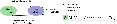
\includegraphics[width=\textwidth]{\chapterdirectory/figure/handling_it/odc2.pdf}
\end{center}
\caption{Overview of ODC\textsuperscript{2}, as seen in \cite{doi:10.1002/cpe.3172}.}%
\label{fig:handling_it:odc2}
\end{figure}

\cite{doi:10.1002/cpe.3172} presents ODC\textsuperscript{2} (On-Demand Coherent
Cache), a strategy to limit the interference of cache coherence on the
execution of real-time software (see Figure~\ref{fig:handling_it:odc2}). The
general idea is to have software delimit sections during which they access
shared data (\textit{Shared Mode}), and to have that shared data be evicted
from the cache as soon as the software leaves the section (\textit{Restore
Procedure}). Any new data loaded during Shared Mode is marked as being
\textit{shared} in the cache line, making their Shared data cannot be accessed
outside of these sections, which makes the code outside these coherence enabled
sections (called \textit{Private Mode}), much simpler to analyze.

A follow-up paper, \cite{Py2015.1}, performs the WCET analysis of some well
established algorithms (Dijkstra algorithm, Fast Fourier Transform, Matrix
Multiplication) by modifying an existing WCET computation framework (OTAWA) to
add support to ODC\textsuperscript{2}. The resulting WCET is compared with the
ones obtained when using no caches, when using \textit{Magic} (cache coherence
without any cost, which represents the best theoretical performance), and an
approach that simply invalidates the full cache upon entering any
synchronization point. The results show, somewhat unsurprisingly,
ODC\textsuperscript{2} obtains a lower computed WCET than the other approaches,
\textit{Magic} excepted.

\stopallthesefloats{}

\subsection{Dynamic Verification of Cache Coherence}
\begin{figure}
\begin{center}
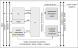
\includegraphics[width=0.7\textwidth]{\chapterdirectory/figure/handling_it/dynamic_verification.pdf}
\end{center}
\caption{Overview of the altered cache, as seen in \cite{Cantin2004DynamicVO}.}%
\label{fig:handling_it:dynamic_verification}
\end{figure}

\cite{Cantin2004DynamicVO} proposes a strategy to implement fault detection in
cache coherence systems, addressing both permanent and temporary issues by
adding hardware (See Figure~\ref{fig:handling_it:dynamic_verification}) that
replicates a simplified version of the cache coherence logic and tests it for
consistency with the real one.

The approach proposed by \cite{Cantin2004DynamicVO} recommends the addition
of a new interconnect dedicated to the validation of the cache coherence
protocol, to avoid disrupting the existing one. This new interconnect is solely
used by caches to broadcast that they entered a stable state for a given memory
element so as to allow the other caches to check that their local state for that
memory element is not in conflict with the broadcasted one. For example, if a
cache broadcasts that it has reached the $M$ state for a memory element, then
all other caches seeing that broadcast would test that they do not have that
memory element in any state other than $I$.

This new verification performed on each cache partaking in the coherence
protocol requires the addition of some hardware to each cache. In addition to
checking for consistency with the other caches through broadcasts, this new
hardware maintains a simplified version of the coherence state of each memory
element. It does not incorporates transient states and, since it only considers
state changes and whether they allow a given instruction to be performed, the
resulting coherence protocol is that of one operating on an atomic interconnect
with atomic operations (such as the one in Section~\ref{sec:intro_to_msi}).
In effect, the simplified protocol only sees events once the transaction they
were part of has been completed. At that point, it receives address, event,
initial and final stable state and compares these with its own record. To detect
timeout issues, a watchdog is also added to the caches.

Thus, while it requires rather complex hardware modifications,
\cite{Cantin2004DynamicVO} does provide a way to detect the occurrence of errors
in the cache coherence protocol's behavior.

\stopallthesefloats{}

% Configuration, lock, set as uncacheable.

\section{By Accepting It}
\label{sec:rel_work:handling_it:accepting_it}
The most common approach to the analysis of interference in caches relies on
the static analysis and abstract interpretation approach originating from
\cite{10.1023/A:1008186323068}, which categorized accesses to caches depending
on whether they always found the value, never did, or if that could not be
determined. This was then taken into account account for the computation of the
WCET. The publications that followed usually propose the addition of a new
categorization, or remark on the incorrectness or incompleteness of the way
these categorizations evolve during the analysis of the program's CFG, and
propose corrections for mistakes made on previous attempts at doing so (up to,
and including, what has been presented in \cite{10.1023/A:1008186323068}).
While otherwise prevalent, this particular approach is not the one focused on in
this thesis, and thus only very few of these papers have been included in this
section. Readers interested in learning more about this subject are encouraged
to read \cite{10.1145/3290367}, and especially its well presented related works
section.

\subsection{Instruction Cache Analysis}
Most papers handling WCET analysis on multi-cores only consider instruction
caches, bypassing the need to address cache coherence by indicating that
instructions cannot be modified. While this makes them slightly outside the
scope of this thesis, the sheer prevalence of this restriction in WCET papers
would make their complete omission feel amiss.


\stopallthesefloats
\subsubsection{WCET analysis}
\begin{figure}[hbt]
\centering
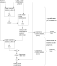
\includegraphics[width=0.65\columnwidth]{\chapterdirectory/figure/handling_it/bypass_to_wcet.pdf}
\caption{%
Overview of the strategy presented in \cite{10.1109/RTSS.2009.34} (taken
from the paper)
}
\label{fig:handling_it:bypass_to_wcet}
\end{figure}

\cite{10.1109/RTSS.2009.34} proposes a way to compute WCET for multi-core
architectures, with considerations for shared instruction caches with multiple
levels of hierarchy. It also tries out a \textit{bypassing scheme}, which
relies on the identification of single-use program blocks within shared
instruction caches to compile programs in a way that reduces interference
between tasks.

The proposed WCET computation strategy is based on existing approaches for
multi-levels instruction caches in single core processors. It uses static
analysis to categorizes all accesses as either: always-miss, always-hit,
first-miss (first access is unknown, but all following accesses will hit), and
not classified (for accesses that fail to be categorized in the other
patterns). This categorization (referred to as \textit{CHMC} in the paper) is
done for every cache level. Furthermore, the likeliness of an access actually
reaching a level is also evaluated and categorized with similar labels (always
acceded, never, always after the first access, unknown). Moving this strategy
to multi-core processors is indicated as having the potential of changing some
always-hit and first-miss into first-miss and \textit{not classified}. Accesses
made by different tasks on the same level where the categorization indicates
that the access is not \textit{never} done are considered as interfering with
one another (regardless of when the accesses are made). This is then used to
re-evaluate the hit/miss categorization so that it has the interference taken
into account. The result of the interference identification analysis is referred
to as \textit{C}ache block \textit{C}onflict \textit{N}umber. To improve the
precision of the result, the possibility of having code shared among tasks
(such as libraries) is taken into account. An overview of the whole process for
a given cache level $\ell$ is shown in
Figure~\ref{fig:handling_it:bypass_to_wcet}.

The decisions made in what to cache generally follow the
locality of reference principle, where the proximity of elements in memory is
assumed to translate to a proximity is usage times, and that processors
receptively access the same elements within short time periods. In
\cite{10.1109/RTSS.2009.34}, static analysis is used to find elements which are
only used once (called \textit{S}tatic \textit{S}ingle \textit{U}sage), in
order to avoid having them pollute caches and risk being considered as a source
of interference needlessly. This relies on a bypass mechanism, that allows
fetching data without altering the caches: if it is not found within any cache,
the value is retrieved but not added to any cache; if it is found within a
cache, the caches in-between do not get any copy, and the copy that was used is
not updated to indicate a recent access.
\stopallthesefloats


\stopallthesefloats

\subsubsection{Unified WCET Analysis Framework}
\begin{figure}
\centering
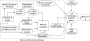
\includegraphics[width=\columnwidth]{\chapterdirectory/figure/handling_it/chattopadhyay_wcet.pdf}
\caption{%
Overview of the strategy presented in \cite{10.1145/2584654} (taken from the
paper)
}
\label{fig:handling_it:chattopadhyay}
\end{figure}
\cite{10.1145/2584654} presents a framework for WCET analysis on multi-core
platforms, which distinguishes itself from other solutions by the number of
features it takes into consideration. Indeed, the framework accounts for shared
caches, pipelines, and branch prediction. It also does not require the
assumption of a timing-anomaly-free architecture. An architecture free of
timing anomalies are architectures for which performing an operation faster on
a core cannot result in a longer execution time for the program compared to if
that operation took longer. The oppose would, for example, if the instruction
activates cache coherence mechanisms which would not have been necessary if the
in faster execution of that instruction. Readers interested in more possible
causes for timing anomalies are encouraged to read
\cite{DBLP:conf/wcet/ReinekeWTWPEB06}).
Figure~\ref{fig:handling_it:chattopadhyay} provides an overview of the
approach.  The assumptions that it does are as follow: use of a TDMA-based
round-robin arbitration policy, cores each have a private L1 cache. Data and
instructions are assumed to be fully separated (separate caches, separate
buses). Only instruction caches are taken into account (no cache coherence, no
possibility of modifications). Caches are assumed to be non-inclusive and to
use the LRU replacement policy.

The approach analyzes the WCET for each core separately.  Using abstract
interpretation, memory accesses are categorized according to whether they
always hit, always miss, or are marked as being unclassified. This is done for
both the L1 and L2 caches. The L2 cache can be a shared one, in which case
accesses susceptible to inter-core interference may move from always hits to
unclassified. This inter-core interference appears to be the only considered
direct interference from other cores, due to the assumptions made on the
architecture. Speculative execution, the result of branch prediction, may also
have effects on the contents of the L1 and L2 caches, as well as the pipeline's
behavior. A model of the shared bus's TDMA is taken into account when creating
the pipeline's model, adding a latency to certain stages. This pipeline model
creation process appears to be fairly complex, proceeding in an iterative
manner to compute the WCET of each basic computation block. Having the WCET of
each basic block, a model of the branch prediction mechanics and that of the
TDMA are used in the definition an linear optimization objective that will
return the WCET of the whole program.


\stopallthesefloats
\subsection{Data Cache Analysis}
\subsubsection{Bypass Heuristics}
\cite{lesage:inria-00531214} uses a similar approach to
\cite{10.1109/RTSS.2009.34}, this time focusing on data caches instead. Cache
coherence protocols are not considered. Indeed, all accesses to shared data is
assumed to bypass private caches (something that could be implemented by
\cite{bansal2019cache}, for example) and all shared-caches are assumed
to be write-through. Data and instructions are assumed to not interfere with
each other. In effect, the main change from what is presented in
\cite{10.1109/RTSS.2009.34} is how accesses to a memory bock are determined:
in the case of an instruction cache, a single instruction always points to
the same memory blocks; whereas in data caches, the relation between instruction
and memory block is murkier, as addresses may be aliased. This makes the
detection of Static Single Usage cache blocks, which were the target of bypass
mechanisms in \cite{10.1109/RTSS.2009.34}, much more complex. Multiple
heuristics on which elements to bypass at shared cache level $\ell$ are
provided: any instruction for which none of the targeted memory references have
statically been detected to be leading to a sure hit in $\ell$ in the future;
any instruction for which the target cannot be statically computed, in order to
increase determinism; and one that bypasses any access of a task until it only
occupies a given number of cache ways, which allows for conflict reduction
through control of the maximum occupied space by each task.


\subsubsection{Write-Back Data Caches}
\cite{10.1145/3139258.3139269} tackles the issue of WCET computation in
multi-core processors that use data (or unified) shared caches with write-back
policies. Although not explicitly stated in the paper, this approach does not
consider separate caches of the same hierarchy: all caches are shared by all
cores that could access the data they contain. Ergo, no cache coherence, but a
cascade of non-inclusive shared caches.

In addition to the standard categorization of a cache line in a particular
cache level (always hits, never hits, and so on\ldots), the \textit{dirtiness}
is also modeled. The possible values are: dirty (i.e.~has been written to, but
changes were not yet propagated), clean, or possibly dirty. The main challenge
is then to estimate when the write back will occur.
\cite{10.1145/3139258.3139269} indicates how to take this new attribute into
account when performing the usual cache static analysis, and the constraints it
adds to the linear optimization problem representation of the WCET computation.




\stopallthesefloats
\section{Conclusion}
\section{Conclusion}
This chapter has shown how UPPAAL's model checking capabilities can be exploited
to analyze the interference caused by cache coherence on the model from
Chapter~\ref{cha:modeling_cache_coherence}.

This analysis starts by a computation of the WCET for each program. Useful in
itself, this analysis is extended by that of the WCET for these programs with
the architecture in different configurations in order to extract more
information about how much of the execution time is caused by interference.

In order to more precisely understand what determine the WCET and to provide
the user with information about elements of the program that can directly be
manipulated, the analysis proceeds by an categorization of the accuracy of each
instruction. This indicates which instructions are unaffected by the
interference, which instructions are always time-consuming, and which
instructions take a varying amount of time depending on the execution. By
looking at the accuracy of all accesses made on each memory element, patterns
for these instructions of varying execution time can sometimes be found, which
results in a more predictable system.

The determining factor for the accuracy of instructions is then properly
defined. This corresponds to a categorization of all external queries depending
on their effects on the permissions held by a cache, and whether a loss of
permission led to an instruction taking additional time. Thus, three categories
of interference are defined: minor (no change of permission, but loss of time
due to query processing), demoting (loss of writing permission), and expelling
(loss of all permissions).

Finally, analyses are performed in order to determine how each instruction
interfere with the other instructions. This results in a graph showing, for
each instruction, which instruction can generate interference that will
directly impact it, the category of this interference, and whether this
interference occurs on all possible executions or not.

This provides the user with a clear understanding of the causes and effects of
cache coherence interference on the programs' instructions, opening the way to
finding means of mitigation for this interference.

